\documentclass[a4paper,12pt]{article}

\usepackage{amsmath,amssymb,amsthm,tikz}
\usetikzlibrary{calc,arrows.meta}
\usepackage[margin=20mm]{geometry}

\setlength{\parindent}{0pt}

\begin{document}\thispagestyle{empty}

\begin{center}
{\Large Sample Assignment 4. Discussed on 2020-10-05,} 
{\em Not graded} 
\end{center}

\vspace{10pt}
{\bf Question 1 (Pointer structure).}\\ 
Given the starting state 
(shown in the image) and the pseudocode, draw the end-state 
after the pseudocode is run. 

\vspace{10pt}
\begin{tabular}[t]{@{}ll@{}} 
\begin{minipage}[t]{0.68\columnwidth}
Initial state of the pointers/nodes:
\begin{center}
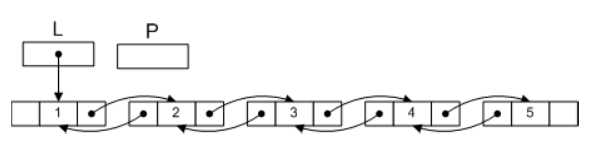
\includegraphics[width=3.5in]{assignment04-pointers/sample-assignment04-pointers.png}
\end{center}

\end{minipage} &
\begin{minipage}[t]{0.25\columnwidth}

The structure of a single node:

\begin{center}
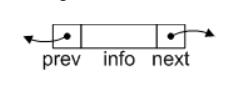
\includegraphics[width=1.5in]{assignment04-pointers/sample-assignment04-structure.png}
\end{center}


\end{minipage}
\end{tabular}


\[
\begin{array}{r l}
1 & P = L \\
2 & P = P \rightarrow \textit{next} \\
3 & P = P \rightarrow next \\
4 & P \rightarrow prev = P \rightarrow next \rightarrow next \\
5 & \text{\textbf{if\ }} P \rightarrow info \geq L \rightarrow info\\
6 & \hspace{.5cm} P \rightarrow next = L \rightarrow next\\
7 & \text{\textbf{else\ }}\\
8 & \hspace{.5cm} L \rightarrow next = P \rightarrow next\\
\end{array}
\]




\end{document}



